An alternative to the Gaussian processes provide the Student-t-processes \cite{Shah_14}. They can be regarded as a generalized Gaussian process. Assuming an inverse Wishart prior for the kernel of a Gaussian process will result in a Student-t process. Due to this, we can also think of the Student-t process as a prior over functions, that is non-parametric. Also belonging to the family of elliptical processes, the Student-t process ($\mathcal{TP}$) offers more robustness to outliers inherent to the process, due to the broader flanks of the Student-t distribution. It is the most general elliptically symmetric process for which analytical marginal and predictive distributions exist. While some argue \cite{Shah_14}, that the predictive covariances of a Gaussian process do not depend on the training observations, the predictive covariances from a Student-t process do depend on training observations. Deriving the Student-t process, we will start with a Wishart process $W_n(\nu,K)$. The Wishart distribution is a distribution over the set of real-valued symmetric matrices, of size $n\times n$, that are positive definite $\Pi(n)$. The density function is
\begin{subequations}%Wishart distribution
	\label{eq:}
	\begin{align}
	\Sigma \sim W_n(\nu,K) \text{, if }         \label{eq:Wishart Distribution} \\
	p(\Sigma) = \Big(|K|^{\nu/2}2^{\nu n/2} \Gamma_n(\nu/2)\Big)^{-1}|\Sigma|^{(\nu-n-1)/2} exp \Big(-\frac{1}{2}tr(K^{-1}\Sigma)\Big)         \label{eq:Wishart distribution definition}
	\end{align}
\end{subequations}
with $\nu > n-1,\text{ } \nu \in \mathbb{R}_+$. This definition exhibits the marginalisation property, just like a GP. But since for $\nu \to \infty$ almost surely $\nu^{-1}\Sigma \to K$, thereby loosing the usefulness of the process. This property is not exhibited in the inverse Wishart process ($Iw_n(\nu, K)$) \cite{Dawid_1981}.
\begin{subequations}%Inverse Wishart Distribution
	\label{eq:}
	\begin{align}
	\Sigma \sim IW_n(\nu,K) \text{ if }         \label{eq:Inverse Wishart distribution} \\
	p(\Sigma) = \Big(\frac{|K|^{(\nu+n-1)/2}}{2^{(\nu+n-1)n/2}\Gamma_n((\nu+n-1)/2)}\Big)^{-1}|\Sigma|^{-(\nu+n-1)/2} exp \Big(-\frac{1}{2}tr(K\Sigma^{-1})\Big)         \label{eq:Inverse Wishart distribution definition}
	\end{align}
\end{subequations}
This formulation requires $\nu > 2$ and $\mathbb{E}[\Sigma] = (\nu-2)^{-1}K$, for the mean and the covariance to exist. Both Wishart distributions place prior mass on every possible matrix $\Sigma$ stemming from the set $\Pi(n)$. It was also previously shown, that the Inverse Wishart distribution is consistent under marginalization. Any submatrix $\Sigma_{11}$ will be $Iw_{n1}(\nu_1K-\Sigma_{11})$ distributed. With this, we can define a Inverse Wishart Process analogous to a Gaussian process with a base kernel $k:\mathcal{X} \times \mathcal{X}\to \mathbb{R}$
\begin{equation}%Inverse Wishart Process
	\sigma \sim \mathcal{IWP}(\nu,k(\cdot,\cdot)).
\label{eq: Inverse Wishart Process}
\end{equation}
If the Inverse Wishart process is applied as prior on the kernel function of a $\mathcal{GP}$, a Student-t process 
\begin{subequations}%Student-t process
	\label{eq:Student-t process}
	\begin{align}
	\sigma \sim \mathcal{IWP}(\nu,k_\theta)         \label{eq:inverse wishart covariance kernel} \\
	\bm{y}|\sigma \sim \mathcal{GP}(\mu, (\nu-2)\sigma)         \label{eq:hierarchical gaussian process with iwp kernel}
	\end{align}
\end{subequations}
generative approach is achieved. We find the data to be Student-t distributed if the density is of the structure
\begin{subequations}%student-t distributed data
	\label{eq:multivariate Student-t distributed data}
	\begin{align}
	\bm{y} \sim \mathcal{MVT}_n(\nu,\bm{\mu},K)         \label{eq:multivariate Student-t shorthand} \\
	p(\bm{y}) = \frac{\Gamma(\frac{\nu+n}{2})}{((\nu-2)\pi)^{\pi/2}\Gamma(\nu/2)}|K|^{-1/2}\Big(1+\frac{(\bm{y}-\bm{\mu})^{\top}K^{-1}(\bm{y}-\bm{\mu})}{\nu-2}\Big)^{-(\nu+n)/2} ,        \label{eq:multivariate Student-t distributed data def}
	\end{align}
\end{subequations}
for which the mean and covariance are given by
\begin{subequations}%mean and cov studt
	\label{eq:mean and cov studt}
	\begin{align}
	\mathbb{E}[\bm{y}] = \mathbb{E}[\mathbb{E}[\bm{y}|\Sigma]] = \bm{\mu}         \label{eq:mean studt} \\
	cov[\bm{y}] = \mathbb{E}[\mathbb{E}[(\bm{y}-\bm{\mu})(\bm{y}-\bm{\mu})^{\top}|\Sigma]]         \label{eq:cov studt}
	\end{align}
\end{subequations}
\cite{Shah_14}. The Student-t process is consistent under marginalisation. As a shorthand, we write $f \sim \mathcal{TP}(\nu, \bm{\mu},K)$ for a joint Student-t process over a finite collection of function values, as a similar counterpart to the Gaussian process over function values \ref{eq:Gaussian_process_function_space_view}. The student-t process generalizes the Gaussian process through the introduction of the degree of freedom parameter $\nu$. For  $\nu \to \infty$ we arrive at a Gaussian process, while at $\nu = 1$ we have a Cauchy process. Analyzing this hyperparameter, we find that it controls how much probability mass lies in the tails of a distribution, directly influencing how large of a variance samples from a Student-t process have compared to a Gaussian process.
\begin{figure}[h!]%Comparison GP and TP samples
	\centering
	\begin{minipage}{0.75\textwidth}
		\centering
		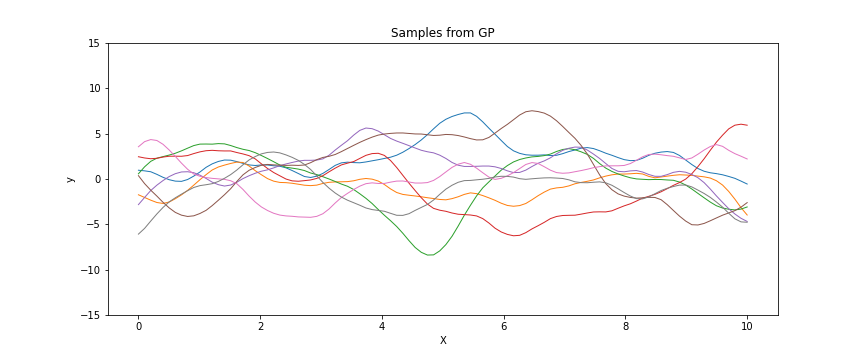
\includegraphics[scale=0.4]{img/05_8/GP_samples.png} % first figure itself
		\caption[GP samples example]{Samples from a GP.}
		\label{fig:GP_samples}
	\end{minipage}\hfill
	\begin{minipage}{0.75\textwidth}
		\centering
		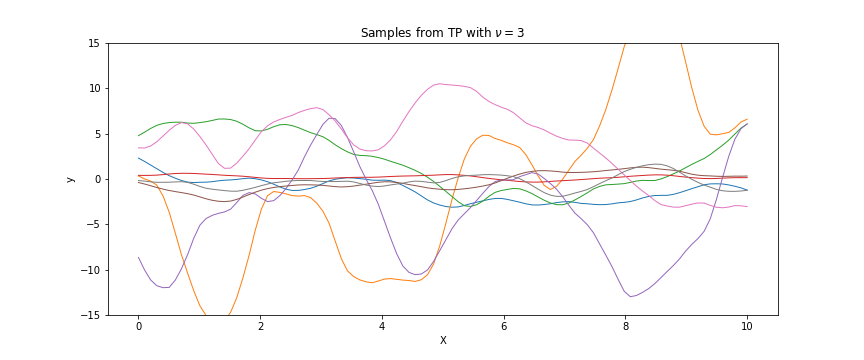
\includegraphics[scale=0.4]{img/05_8/TP_samples.png} % second figure itself
		\caption[TP samples example]{Samples from a TP.}
		\label{fig:TP_samples}
	\end{minipage}
\end{figure}
In figures \ref{fig:GP_samples} and \ref{fig:TP_samples}, the comparison of Gaussian process prior samples (upper) and Student-t (lower) process prior samples are shown. In general the Student-t samples have a broader credibility predictive sample interval compared to the Gaussian process. This leads to a higher tolerance for outliers in the data sets, since the outliers do not impact the covariance as much as with a Gaussian process. A higher parameter $\nu$ leads to a more narrow credibility interval.
After analysing the properties of a Student-t process prior, the conditional distributions can be analyzed. Splitting up a data set into e.g. a test ($\bm{y}_*$) and training ($\bm{y}$) dataset, the respective multivariate Student-t process becomes
\begin{subequations}%multivariate student t conditional distribution
	\label{eq:multivariate student t conditional distribution}
	\begin{align}
	\scriptstyle
	\bm{y}_*|\bm{y} \sim \mathcal{MVT}_{n_*}(\nu+n, K(X_*,X)K(X,X)^{-1}(\bm{y}-\bm{\mu})+\bm{\mu_*},  \nonumber \\
	\scriptstyle
	 \frac{\nu+(\bm{y}-\bm{\mu})^{\top}K(X,X)^{-1}(\bm{y}-\bm{\mu})-2 }{\nu+n-2}(K(X_*,X_*)-K(X_*,X)K(X,X)^{-1}K(X,X_*))) 
	\end{align}
\end{subequations}
with number of datapoints $n_*$ in $\bm{y}_*$ and $n$ in $\bm{y}$ respectively. 